\newpage
\section{Qualità di prodotto}
	
Al fine di garantire una buona qualità di prodotto, il \textit{team\ped{G}} ha individuato dallo standard \textbf{\textit{ISO/IEC 9126\ped{G}}} le qualità che ritiene più importanti durante tutto il ciclo di vita del prodotto \progetto. Per ognuna delle qualità individuate, sono stati definiti obiettivi e metriche coerenti con i livelli di qualità dichiarati.

\begin{figure}[H]
	\centering
	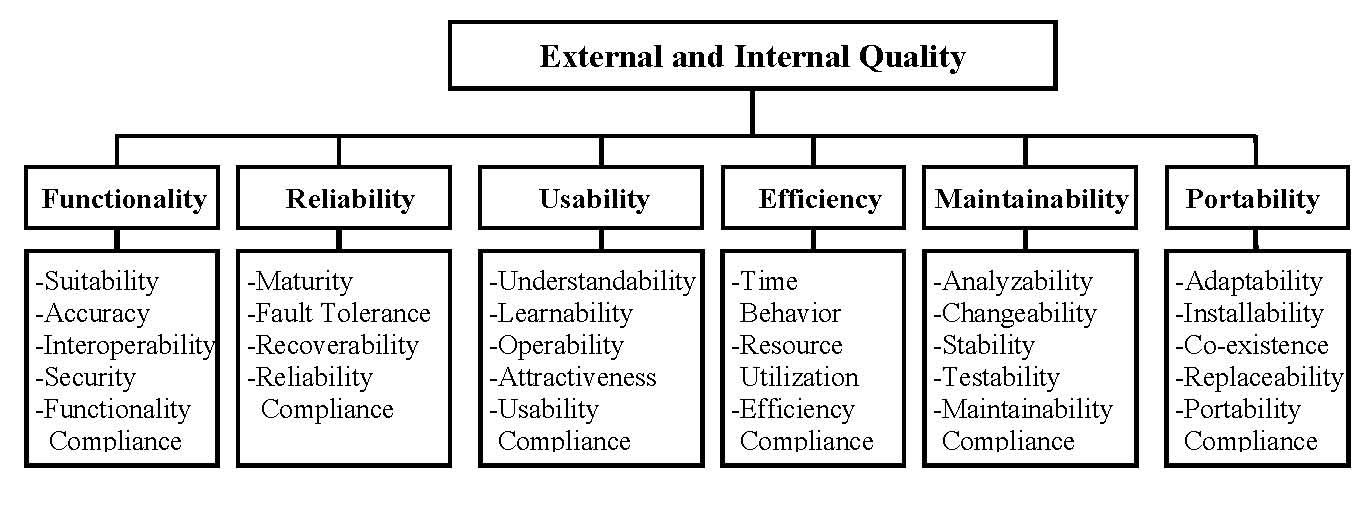
\includegraphics[scale=0.35]{includes/img/9126.png}
	\caption{Standard ISO/IEC 9126}
\end{figure}

Le \textbf{metriche interne} si applicano al software non eseguibile, come ad esempio le specifiche tecniche e il codice sorgente, durante i periodi di progettazione e codifica.
Esse sono specificate nella norma \textbf{\textit{ISO/IEC 9126-3\ped{G}}}.\\
Durante le fasi di sviluppo del software, i prodotti intermedi sono valutati tramite metriche interne che misurano le proprietà intrinseche del prodotto.
Le misure effettuate permettono di prevedere il livello di qualità esterna ed in uso del prodotto finale, in quanto gli attributi interni influenzano le caratteristiche esterne e quelle in uso.
Le metriche interne misurano attributi interni del software e forniscono indicazioni sulle caratteristiche esterne del prodotto finale, tramite l'analisi statica dei prodotti intermedi.
Le metriche interne si applicano anche alla documentazione del prodotto.\\
Le \textbf{metriche esterne} misurano i comportamenti del prodotto software rilevabili dai test, dall'operatività e dall'osservazione durante la su esecuzione, in funzione degli obiettivi stabiliti.
Esse sono specificate nella norma \textbf{\textit{ISO/IEC 9126-2\ped{G}}}.	

\subsection{Definizione degli obiettivi di qualità}

	\subsubsection{Funzionalità}
	Rappresenta la capacità del prodotto nel fornire le funzionalità richieste e soddisfare tutti i requisiti descritti nel documento \textsc{AnalisiDeiRequisiti 3\_0\_0.pdf}.
		
		\paragraph{Obiettivi}
			\begin{itemize}
				\item \textbf{Adeguatezza:} rappresenta la capacità di fornire un appropriato insieme di funzionalità che permettano agli utenti di svolgere determinati task e raggiungere gli obiettivi prefissati.
				\item \textbf{Accuratezza:} rappresenta la capacità di fornire i risultati e gli effetti attesi con il livello di precisione richiesta.
				\item \textbf{Sicurezza:} rappresenta la capacità di proteggere le informazioni ed i dati, in modo che persone o sistemi non autorizzati non possano accedervi.
			\end{itemize}
		
		\paragraph{Metriche}
			\subparagraph{Completezza delle funzioni sviluppate}
			Indica la percentuale di funzionalità sviluppate ritenute complete.
			
			\begin{itemize}
				\item \textbf{fun\ped{Compl}} = numero di funzioni ritenute complete
				\item \textbf{fun\ped{Tot}} = numero di funzioni totali
			\end{itemize}
			
		\begin{table}[H]
			\begin{longtable}{>{\centering\arraybackslash}p{5cm}|>{\centering\arraybackslash}p{5cm} | >{\centering\arraybackslash}p{5cm}}
				\hline
				\rowcolor{Gray}
				\textbf{Metodo di calcolo} & \textbf{Range accettazione} & \textbf{Range ottimale} \\
				\hline
			     \begin{math}
			     \frac{fun\ped{Compl}}{fun\ped{Tot}}*100
			     \end{math} & [90,100] in [0,100]& [90,100] in [0,100] 
			\end{longtable}
			\caption{Completezza delle funzioni sviluppate}
		\end{table}
			
			\subparagraph{Correttezza delle funzioni sviluppate}
			Indica la percentuale di funzionalità sviluppate ritenute corrette.
			
			\begin{itemize}
				\item \textbf{fun\ped{Corr}} = numero di funzioni ritenute corrette
				\item \textbf{fun\ped{Tot}} = numero di funzioni totali
			\end{itemize}
			
			\begin{table}[H]
				\begin{longtable}{>{\centering\arraybackslash}p{5cm}|>{\centering\arraybackslash}p{5cm} | >{\centering\arraybackslash}p{5cm}}
					\hline
					\rowcolor{Gray}
					\textbf{Metodo di calcolo} & \textbf{Range accettazione} & \textbf{Range ottimale} \\
					\hline
					\begin{math}
					\frac{fun\ped{Corr}}{fun\ped{Tot}}*100
					\end{math} & 100 in [0,100]& 100 in [0,100] 
				\end{longtable}
				\caption{Corretezza delle funzioni sviluppate}
			\end{table}
			
			\subparagraph{Accuratezza rispetto alle aspettative}
			Indica la percentuale di risultati conformi alle aspettative.
			
			\begin{itemize}
				\item \textbf{test\ped{Corr}} = numero di test ritenuti corretti
				\item \textbf{test\ped{Tot}} = numero di test totali
			\end{itemize}
			
			\begin{table}[H]
				\begin{longtable}{>{\centering\arraybackslash}p{5cm}|>{\centering\arraybackslash}p{5cm} | >{\centering\arraybackslash}p{5cm}}
					\hline
					\rowcolor{Gray}
					\textbf{Metodo di calcolo} & \textbf{Range accettazione} & \textbf{Range ottimale} \\
					\hline
					\begin{math}
					\frac{test\ped{Corr}}{test\ped{Tot}}*100
					\end{math} & [90,100] in [0,100]& [95,100] in [0,100] 
				\end{longtable}
				\caption{Accuratezza rispetto alle aspettative}
			\end{table}
			
			
			\subparagraph{Controllo degli accessi}
			Indica la percentuale di accessi corretti al sistema.
			
			\begin{itemize}
				\item \textbf{accessi\ped{Succ}} = numero di accessi controllati con successo dal sistema
				\item \textbf{accessi\ped{Tot}} = numero di accessi totali
			\end{itemize}
			
			\begin{table}[H]
				\begin{longtable}{>{\centering\arraybackslash}p{5cm}|>{\centering\arraybackslash}p{5cm} | >{\centering\arraybackslash}p{5cm}}
					\hline
					\rowcolor{Gray}
					\textbf{Metodo di calcolo} & \textbf{Range accettazione} & \textbf{Range ottimale} \\
					\hline
					\begin{math}
					\frac{accessi\ped{Succ}}{accessi\ped{Tot}}*100
					\end{math} & [90,100] in [0,100]& 100 in [0,100] 
				\end{longtable}
				\caption{Controllo degli accessi}
			\end{table}
			
	
	\subsubsection{Affidabilità}
	Rappresenta la capacità del prodotto software di mantenere il livello di prestazione, quando viene utilizzato in condizioni specificate.
		
		\paragraph{Obiettivi}
			\begin{itemize}
				\item \textbf{Maturità:} rappresenta la capacità di evitare che si verifichino errori o siano prodotti risultati non corretti in fase di esecuzione.
				\item \textbf{Tolleranza agli errori:} rappresenta la capacità di mantenere il livello di prestazioni in caso di errori nel software o di violazione nelle interfacce specificate.
			\end{itemize}
		
		\paragraph{Metriche}
			\subparagraph{Chiamate a microservizi corrette}
			Indica il numero di chiamate al microservizio j andate a buon fine.
			
			\begin{itemize}
				\item \textbf{num\ped{CF(MS(j))}} = numero di chiamate al microservizio j fallite o avvenute con successo, ma con t\ped{R(MS(j))} > t\ped{MR(MS(j))} + 0.3*t\ped{MR(MS(j))}, dove t\ped{R(MS(j))} = tempo di risposta del microservizio j e t\ped{MR(MS(j))} = tempo medio di risposta del microservizio j
				\item \textbf{num\ped{CT(MS(j))}} = numero totale di chiamate al microservizio j
			 
			\end{itemize}
			
			\begin{table}[H]
				\begin{longtable}{>{\centering\arraybackslash}p{5cm}|>{\centering\arraybackslash}p{5cm} | >{\centering\arraybackslash}p{5cm}}
					\hline
					\rowcolor{Gray}
					\textbf{Metodo di calcolo} & \textbf{Range accettazione} & \textbf{Range ottimale} \\
					\hline
					\begin{math}
					\frac{num\ped{CF(MS(j))}}{num\ped{CT(MS(j))}}*100
					\end{math} & [90,100] in [0,100]& 100 in [0,100] 
				\end{longtable}
				\caption{Chiamate a microservizi corrette}
			\end{table}
			
		
			\subparagraph{Copertura dei test}
			Indica il livello di copertura dei test.
			
			\begin{itemize}
				\item \textbf{test\ped{P}} = numero di test pianificati
				\item \textbf{test\ped{N}} = numero di test necessari a garantire la copertura richiesta o massima
			\end{itemize}
			
			\begin{table}[H]
				\begin{longtable}{>{\centering\arraybackslash}p{5cm}|>{\centering\arraybackslash}p{5cm} | >{\centering\arraybackslash}p{5cm}}
					\hline
					\rowcolor{Gray}
					\textbf{Metodo di calcolo} & \textbf{Range accettazione} & \textbf{Range ottimale} \\
					\hline
					\begin{math}
					\frac{test\ped{P}}{test\ped{N}}*100
					\end{math} & [80,100] in [0,100] & 100 in [0,100] 
				\end{longtable}
				\caption{Copertura dei test}
			\end{table}
			
			
			\subparagraph{Controllo dei guasti}
			Indica il livello di controllo dei guasti, attraverso il numero di condizioni di errore messe sotto controllo per evitare malfunzionamenti e/o guasti al prodotto.
			
			\begin{itemize}
				\item \textbf{num\ped{CEG}} = numero di condizioni d'errore gestite correttamente
				\item \textbf{num\ped{CEP}} = numero di condizioni d'errore possibili nel sistema
			\end{itemize}
			
			\begin{table}[H]
				\begin{longtable}{>{\centering\arraybackslash}p{5cm}|>{\centering\arraybackslash}p{5cm} | >{\centering\arraybackslash}p{5cm}}
					\hline
					\rowcolor{Gray}
					\textbf{Metodo di calcolo} & \textbf{Range accettazione} & \textbf{Range ottimale} \\
					\hline
					\begin{math}
					\frac{num\ped{CEG}}{num\ped{CEP}}*100
					\end{math} & [80,100] in [0,100] & 100 in [0,100] 
				\end{longtable}
				\caption{Controllo dei guasti}
			\end{table}
			
	
	\subsubsection{Usabilità}
	Rappresenta la capacità di un prodotto software di essere comprensibile, di poter essere studiato e di risultare attraente da parte di un utente sotto determinate condizioni.
	
		\paragraph{Obiettivi}
			\begin{itemize}
				\item \textbf{Comprensibilità:} rappresenta la capacità di permettere all'utente di capire le funzionalità del prodotto software e come poterle utilizzare con successo per svolgere particolari task in determinate condizioni di utilizzo.
				\item \textbf{Operabilità:} rappresenta la capacità di permettere all'utente di utilizzare e controllare il prodotto software.
				\item \textbf{Attrattività:} rappresenta la capacità di risultare piacevole per l'utente.
			\end{itemize}
		
		\paragraph{Metriche}
			\subparagraph{Comprensibilità delle funzionalità offerte}
			Indica la percentuale di funzioni comprensibili agli utenti.
			
				\begin{itemize}
				\item \textbf{num\ped{FC}} = numero di funzionalità comprensibili agli utenti
				\item \textbf{num\ped{FT}} = numero di funzionalità totali offerte
			\end{itemize}
			
			\begin{table}[H]
				\begin{longtable}{>{\centering\arraybackslash}p{5cm}|>{\centering\arraybackslash}p{5cm} | >{\centering\arraybackslash}p{5cm}}
					\hline
					\rowcolor{Gray}
					\textbf{Metodo di calcolo} & \textbf{Range accettazione} & \textbf{Range ottimale} \\
					\hline
					\begin{math}
					\frac{num\ped{FC}}{num\ped{FT}}*100
					\end{math} & [80,100] in [0,100] & [90,100] in [0,100] 
				\end{longtable}
				\caption{Comprensibilità delle funzionalità offerte}
			\end{table}
			
			\subparagraph{Controllo e monitoraggio delle operazioni}
			Indica la capacità del prodotto di monitorare lo stato delle operazioni eseguite.
			
				\begin{itemize}
				\item \textbf{num\ped{FC}} = numero di funzionalità con adeguato controllo e monitoraggio delle operazioni
				\item \textbf{num\ped{FCT}} = numero di funzionalità con controllo totali
			\end{itemize}
			
			\begin{table}[H]
				\begin{longtable}{>{\centering\arraybackslash}p{5cm}|>{\centering\arraybackslash}p{5cm} | >{\centering\arraybackslash}p{5cm}}
					\hline
					\rowcolor{Gray}
					\textbf{Metodo di calcolo} & \textbf{Range accettazione} & \textbf{Range ottimale} \\
					\hline
					\begin{math}
					\frac{num\ped{FC}}{num\ped{FCT}}*100
					\end{math} & [80,100] in [0,100] & [90,100] in [0,100] 
				\end{longtable}
				\caption{Controllo e monitoraggio delle operazioni}
			\end{table}
			
			\subparagraph{Qualità della messaggistica}
			Indica il grado di chiarezza, completezza e correttezza dei messaggi previsti rispetto alle diverse condizioni gestite dal prodotto (ad esempio, il completamento di una funzione, le condizioni di errore, le scelte da effettuare, etc.).
			
			\begin{itemize}
				\item \textbf{num\ped{MC}} = numero di messaggi che risultano chiari, completi e corretti
				\item \textbf{num\ped{MT}} = numero totale di messaggi previsti
			\end{itemize}
			
			\begin{table}[H]
				\begin{longtable}{>{\centering\arraybackslash}p{5cm}|>{\centering\arraybackslash}p{5cm} | >{\centering\arraybackslash}p{5cm}}
					\hline
					\rowcolor{Gray}
					\textbf{Metodo di calcolo} & \textbf{Range accettazione} & \textbf{Range ottimale} \\
					\hline
					\begin{math}
					\frac{num\ped{MC}}{num\ped{MT}}*100
					\end{math} & [70,100] in [0,100] & 100 in [0,100] 
				\end{longtable}
				\caption{Qualità della messaggistica}
			\end{table}
	
	\subsubsection{Efficienza}
	Rappresenta la capacità di un prodotto software di realizzare le funzioni richieste nel minor tempo possibile ed utilizzando nel miglior modo le risorse necessarie.
		
		\paragraph{Obiettivi}
			\begin{itemize}
				\item \textbf{Comportamento rispetto al tempo:} rappresenta la capacità di fornire appropriati tempi di risposta, tempi di elaborazione e quantità di lavoro eseguendo le funzionalità previste.
				\item \textbf{Utilizzo delle risorse:} rappresenta la capacità di utilizzare un appropriato numero e tipo di risposte quando esegue le funzionalità previste.
			\end{itemize}
		
		\paragraph{Metriche}
			
			\subparagraph{Tempo di risposta}
			Indica il tempo medio che intercorre fra la richiesta di una determinata funzionalità e la restituzione del risultato all’utente. L'unità di misura scelta per esprimere il tempo è il \textit{secondo}.
			\begin{itemize}
				\item t\ped{i} = tempo trascorso
				fra la richiesta i di una funzionalità ed il completamento delle operazioni necessarie
				alla restituzione del risultato alla richiesta i
			\end{itemize}
		\begin{table}[H]
			\begin{longtable}{>{\centering\arraybackslash}p{5cm}|>{\centering\arraybackslash}p{5cm} | >{\centering\arraybackslash}p{5cm}}
				\hline
				\rowcolor{Gray}
				\textbf{Metodo di calcolo} & \textbf{Range accettazione} & \textbf{Range ottimale} \\
				\hline
				\begin{math}
				\frac{\sum_{i=1}^{n}(t\ped{i})}{n} 
				\end{math} & [0,10] & [0,4]
			\end{longtable}
			\caption{Tempo di risposta}
		\end{table}
			
			\iffalse
			\subparagraph{Tempo di risposta}
			Indica il tempo medio di risposta per una chiamata ad un microservizio j. La seguente formula viene usata per ridurre gli errori nel conteggio del valore medio su un insieme molto grande di dati.
			
			\begin{itemize}
				\item \textbf{MS(j)} = microservizio j
				\item \textbf{tI\ped{(i)(MS(j))}} = tempo di inizio della i-esima interazione col microservizio j
				\item \textbf{tF\ped{(i)(MS(j))}} = tempo di fine della i-esima interazione col microservizio j  
			\end{itemize}
			
			\begin{table}[H]
				\begin{longtable}{>{\centering\arraybackslash}p{5cm}|>{\centering\arraybackslash}p{5cm} | >{\centering\arraybackslash}p{5cm}}
					\hline
					\rowcolor{Gray}
					\textbf{Metodo di calcolo} & \textbf{Range accettazione} & \textbf{Range ottimale} \\
					\hline
					\begin{math}
					\frac{1}{tI\ped{(i)(MS(j))}-tI\ped{(0)(MS(j))}}*(\sum_{1}^{n}(tF\ped{(2i)(MS(j))} - 4*tF\ped{(2i+1)(MS(j))} + tF\ped{(2i+2)(MS(j))}) 
					\end{math} con n = numero di interazioni col microservizio j &\begin{math}trisp(ms(j)) >= tmediorisp(ms(j)) + 0.3*tmediorisp(ms(j)) \end{math}& trisp(ms(j)) >= tmediorisp(ms(j)) + 0.05*tmediorisp(ms(j))
				\end{longtable}
				\caption{Tempo di risposta}
			\end{table}
			\fi
	
	\subsubsection{Manutenibilità}
	Rappresenta la capacità di un prodotto software di essere modificato. Le modifiche possono includere correzioni o adattamenti del software a modifiche negli ambienti, nei requisiti e nelle specifiche funzionali.
	
		\paragraph{Obiettivi}
			\begin{itemize}
				\item \textbf{Analizzabilità:} rappresenta la capacità di poter effettuare la diagnosi sul software ed individuare le cause di errori o malfunzionamenti.
				\item \textbf{Modificabilità:} rappresenta la capacità di consentire lo sviluppo di modifiche al codice, alla progettazione e alla documentazione.
				\item \textbf{Stabilità:} rappresenta la capacità di evitare effetti non desiderati a seguito di modifiche al software.
				\item \textbf{Testabilità:} rappresenta la capacità di consentire la verifica e la validazione del software modificato, cioè di eseguire test.
			\end{itemize}
	
		\paragraph{Metriche}

			
			\subparagraph{Impatto delle modifiche}
			Indica la percentuale di modifiche effettuate in risposta a failure, le quali hanno portato all’introduzione di nuove failure in altre componenti del sistema.
			
			\begin{itemize}
				\item \textbf{num\ped{FRNF}} = numero di failure risolte con l’introduzione di nuove failure
				\item \textbf{num\ped{FR}} = numero di failure risolte
			\end{itemize}
			
			\begin{table}[H]
				\begin{longtable}{>{\centering\arraybackslash}p{5cm}|>{\centering\arraybackslash}p{5cm} | >{\centering\arraybackslash}p{5cm}}
					\hline
					\rowcolor{Gray}
					\textbf{Metodo di calcolo} & \textbf{Range accettazione} & \textbf{Range ottimale} \\
					\hline
					\begin{math}
					\frac{num\ped{FRNF}}{num\ped{FR}}*100 
					\end{math} & [0,25] in [0,100] & [0,10] in [0,100]
				\end{longtable}
				\caption{Impatto delle modifiche}
			\end{table}
			
		
	
	\subsubsection{Portabilità}
	Rappresenta la capacità di un prodotto software di poter essere trasportato da un ambiente ad un altro.
		
		\paragraph{Obiettivi}
			\begin{itemize}
				\item \textbf{Adattabilità:} rappresenta la capacità del prodotto di essere adattato a differenti ambienti, senza richiedere azioni specifiche diverse da quelle previste dal software per tali attività.
			\end{itemize}
		
		\paragraph{Metriche}
			\subparagraph{Supporto differenti versioni dei browser}
			Indica la percentuale di versioni dei browser supportate.
			
			\begin{itemize}
				\item \textbf{num\ped{VSupp}} = numero delle versioni dei browser supportati
				\item \textbf{num\ped{VTot}} = numero totale delle versioni che devono essere supportate
			\end{itemize}
			
			\begin{table}[H]
				\begin{longtable}{>{\centering\arraybackslash}p{5cm}|>{\centering\arraybackslash}p{5cm} | >{\centering\arraybackslash}p{5cm}}
					\hline
					\rowcolor{Gray}
					\textbf{Metodo di calcolo} & \textbf{Range accettazione} & \textbf{Range ottimale} \\
					\hline
					\begin{math}
					\frac{num\ped{VSupp}}{num\ped{VTot}}*100
					\end{math}  & [90,100] in [0,100]  & 100 in [0,100] 
				\end{longtable}
				\caption{Supporto differenti versioni dei browser}
			\end{table}
	